\subsection{USUÁRIOS E AUTENTICAÇÃO}

Para controlar a visibilidade de informações no sistema desenvolvido, implementou-se um sistema de usuários. A melhoria consistiu na:

\begin{enumerate}
	\item Criação de tabela de usuários no banco de dados;
	\item Associação da tabela ``configuracao'' com a tabela de usuários, para que fosse possível armazenar o usuário responsável por cada configuração;
	\item Criação da tela de login na interface web;
	\item Criação das rotas de cadastro e \textit{login} no servidor
	\item Criação do \textit{middleware} de autenticação
	\item Criação do \textit{middleware} de validação da configuração
\end{enumerate}

\subsubsection{Adaptação do banco de dados}
A aplicação dos itens 1 e 2 foi realizada diretamente no banco de dados, através da criação da tabela mencionada e a chave estrangeira possibilitando a associação de cada usuário a múltiplas configurações. Após estas alterações, o diagrama entidade relacionamento do banco de dados passa a ser representado pela figura \ref{fig:er_atualizado}.

\begin{figure}[!htb]
	\centering
	\caption{Modelo Entidade-Relacionamento com adição da tabela de usuários}
	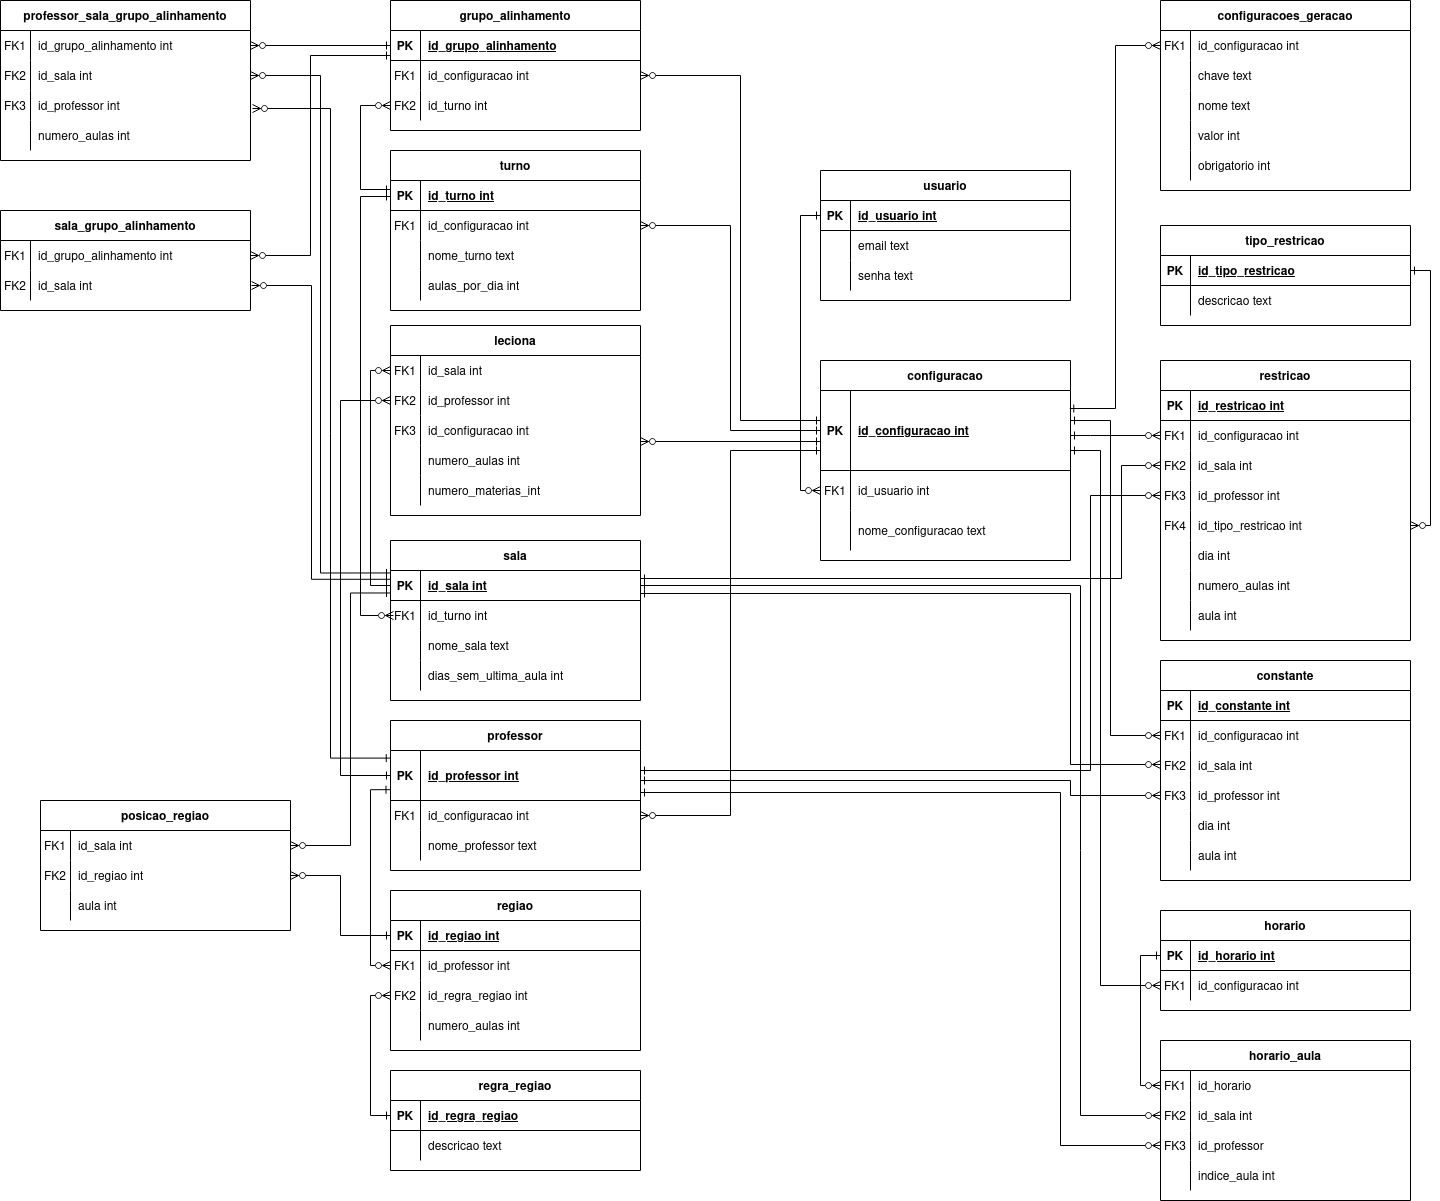
\includegraphics[width=0.65\textwidth]{./dados/figuras/er_horario_com_usuario}
	\fonte{Autor}
	\label{fig:er_atualizado}
\end{figure}

\subsubsection{Tela de login}
Como pode ser visto na figura \ref{fig:login}, desenvolveu-se uma tela simples de \textit{login}, a qual também desempenha a função de cadastro de novos usuários.

\begin{figure}[!htb]
	\centering
	\caption{Tela de Acesso}
	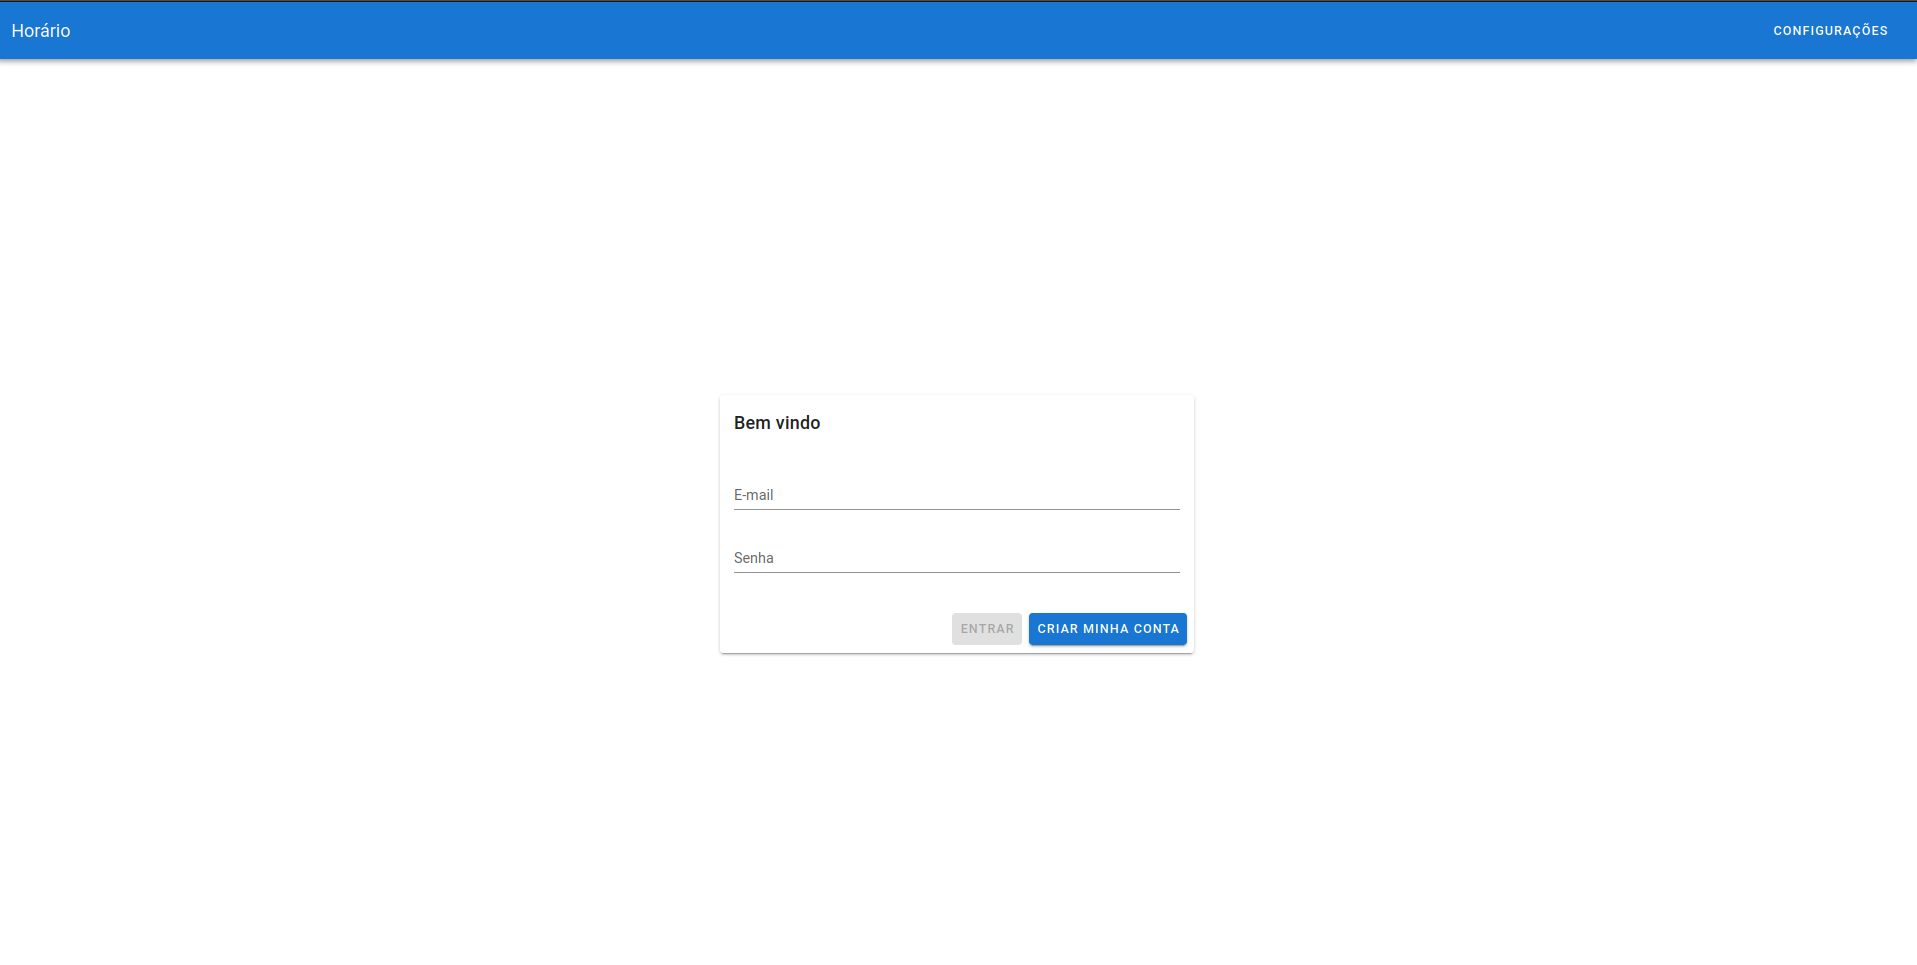
\includegraphics[width=1\textwidth]{./dados/figuras/telaLogin}
	\fonte{Autor}
	\label{fig:login}
\end{figure}
\pagebreak

\subsubsection{Rotas de autenticação}
Para a implementação das rotas de cadastro e \textit{login}, utilizou-se além do \textit{framework ExpressJS}, os pacotes JWT (\textit{Json Web Token}) e \textit{bcrypt}. O pacote JWT é utilizado para gerar \textit{tokens}, que são enviados para a interface web e podem ser utilizados para autenticar os usuários; já o \textit{bcrypt} é utilizado para gerar e validars as \textit{hashes} das senhas dos usuários, para que nunca sejam armazenadas senhas em texto pleno no banco de dados.

A função utilizada pela nova rota de cadastro pode vista na figura \ref{fig:metodoCadastro}. A função ``register'' realiza a validação dos parâmetros, e cria um usuário no banco de dados, caso já não exista outro com o mesmo e-mail. Além disso, a função retorna um \textit{token} JWT para a interface web, para que seja possível verificar a autenticidade das próximas requisições realizadas pelo usuário. 

\begin{figure}[!htb]
	\centering
	\caption{Método de Cadastro}
	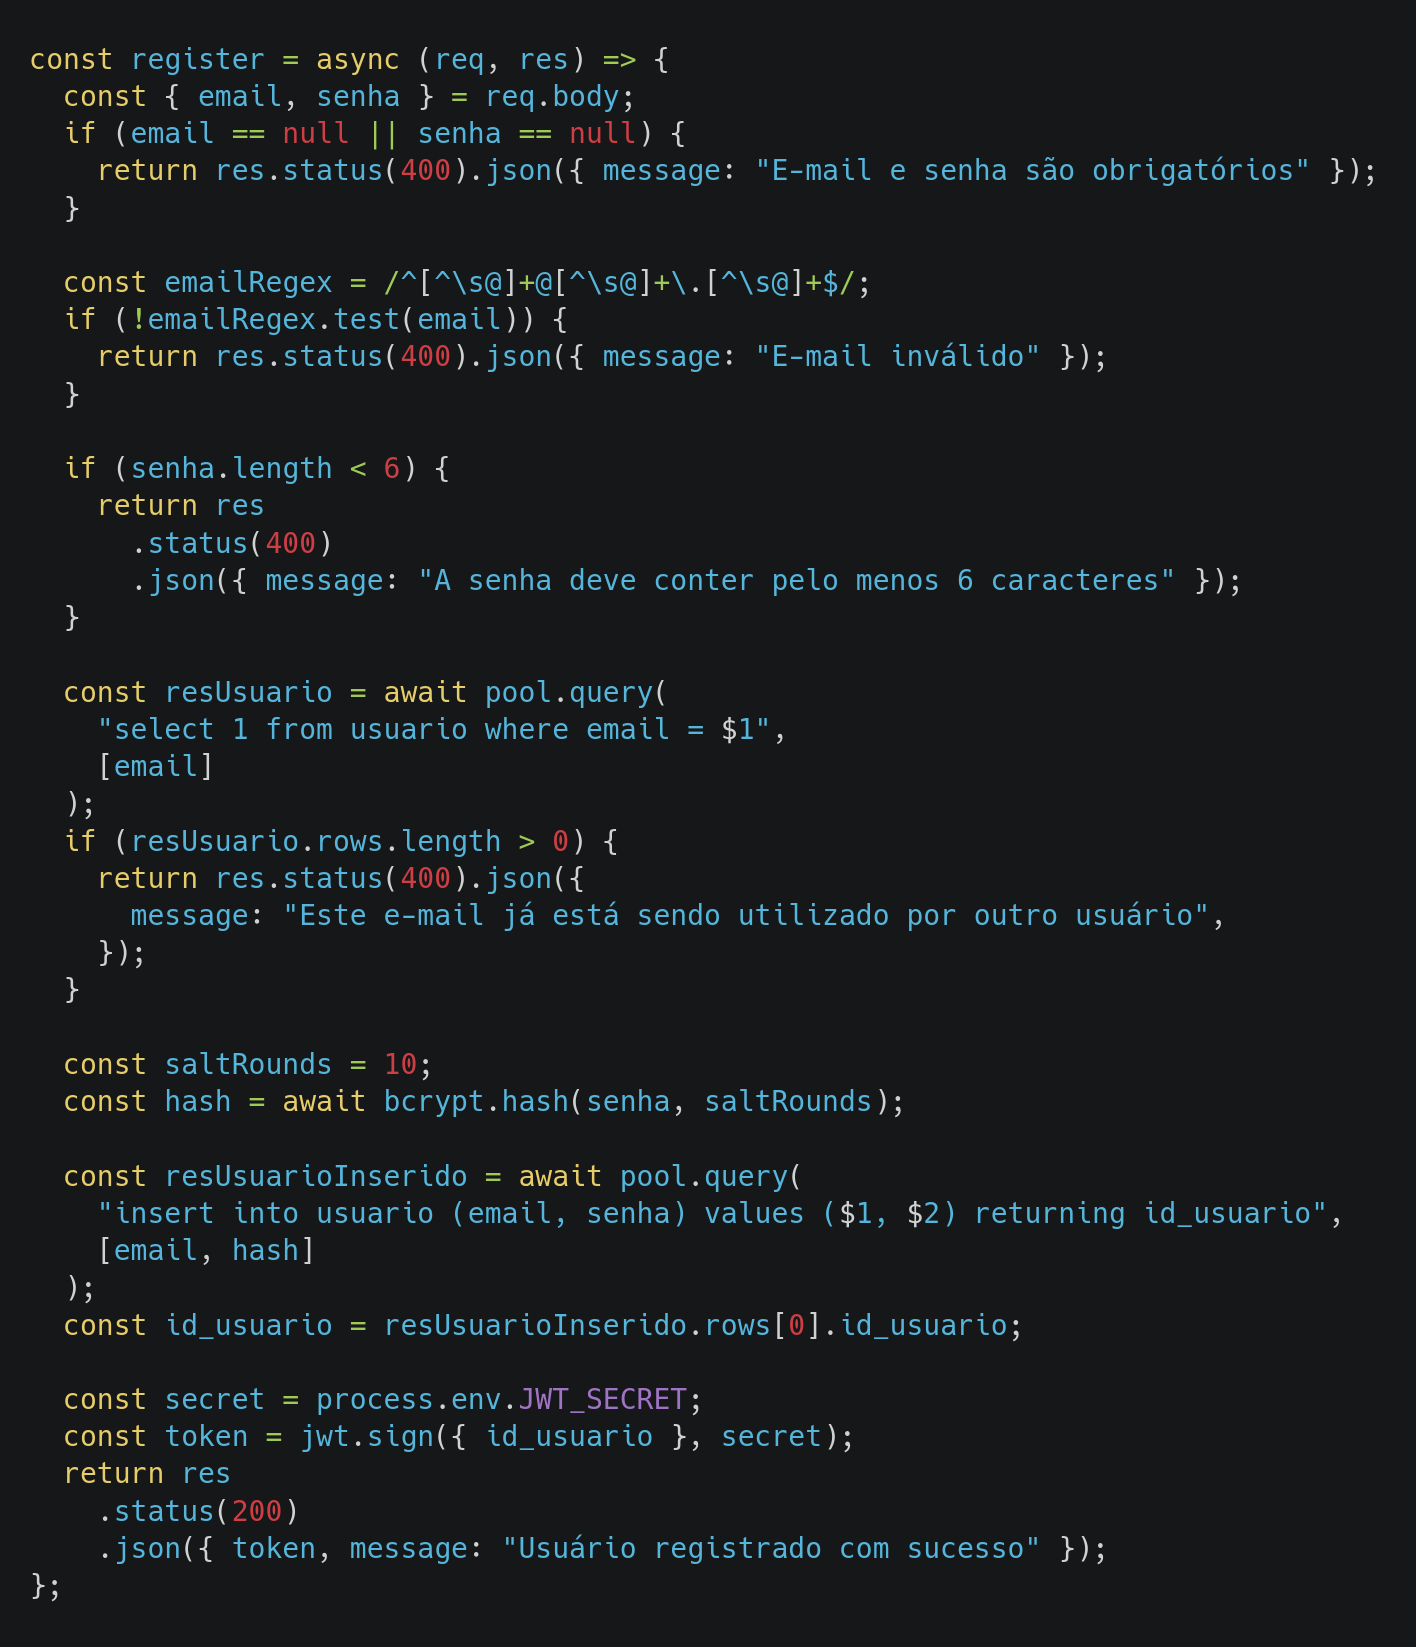
\includegraphics[width=0.8\textwidth]{./dados/figuras/register}
	\fonte{Autor}
	\label{fig:metodoCadastro}
\end{figure}
\pagebreak

A função de \textit{login}, visível na figura \ref{fig:metodoLogin} é similar, realizando validação dos parâmetros, autenticação do usuário através da comparação de senhas utilizando o pacote \textit{bcrypt} e geração de \textit{token} JWT. Vale citar que em ambas as rotas de autenticação, é inserido no \textit{payload} do \textit{token} o identificador do usuário, que posteriormente pode ser utilizado pelos \textit{middlewares} para a realização de validações.

\begin{figure}[!htb]
	\centering
	\caption{Método de Login}
	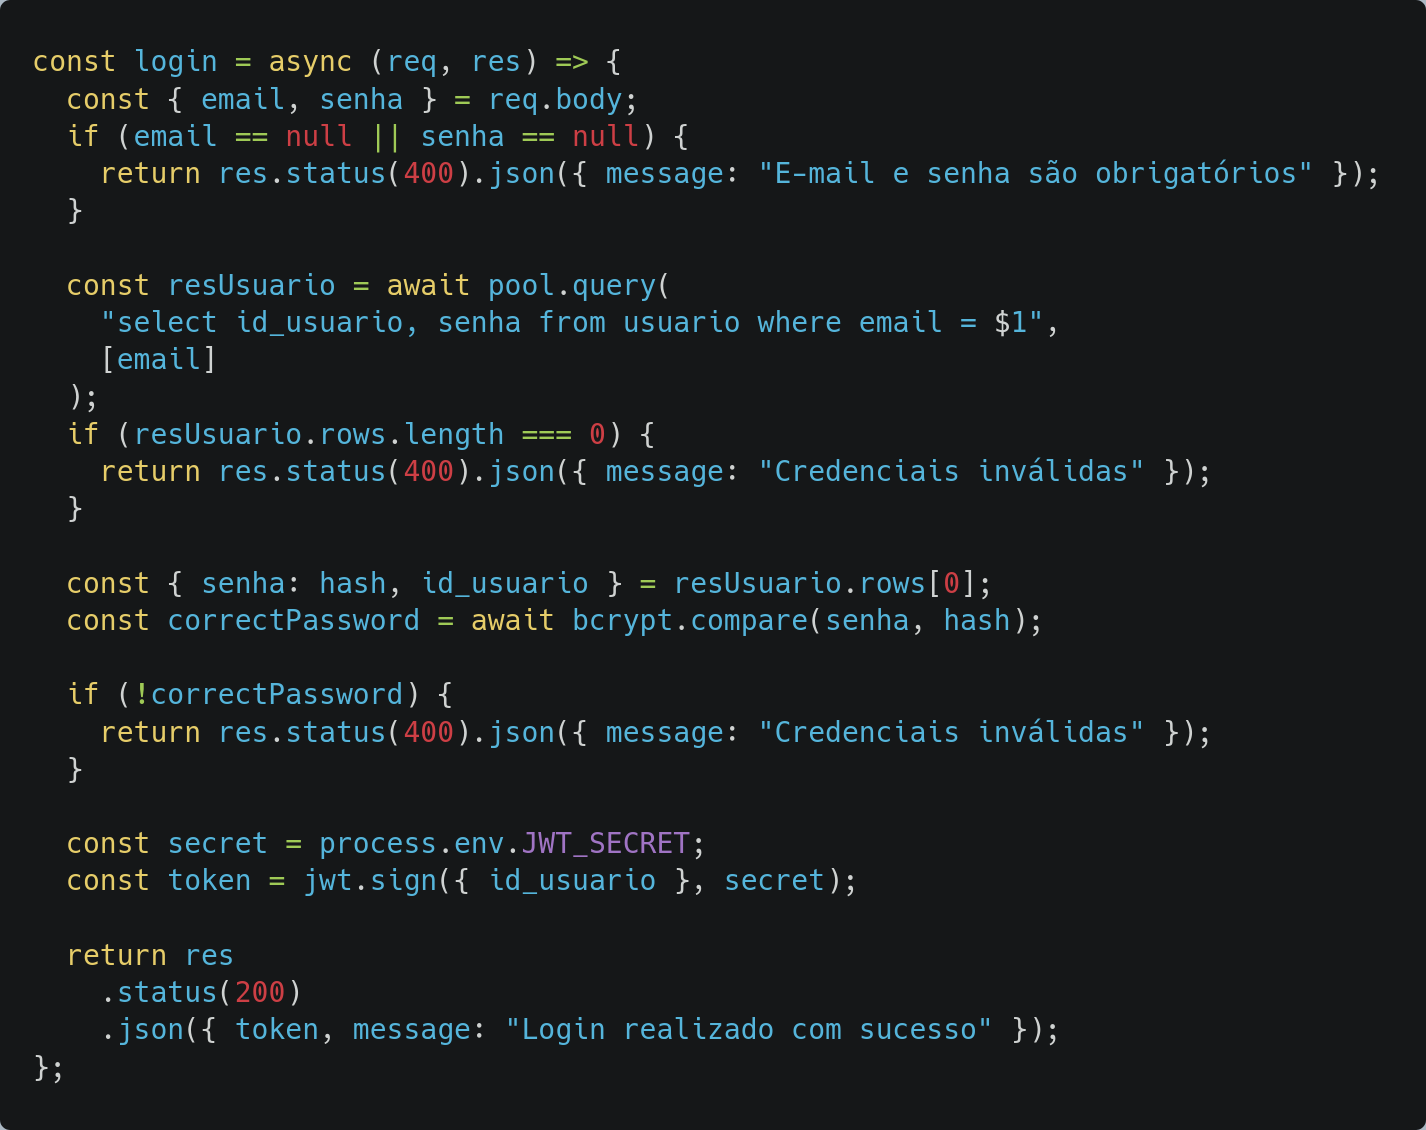
\includegraphics[width=0.8\textwidth]{./dados/figuras/login}
	\fonte{Autor}
	\label{fig:metodoLogin}
\end{figure}
\pagebreak

\subsubsection{Middlewares}
Foram criadas duas funções \textit{middleware} relacionadas aos usuários. A primeira é responsável por assegurar que apenas usuários propriamente autenticados tenham acesso aos recursos protegidos do sistema. Como pode ser visto na figura \ref{fig:auth}, essa verificação é realizada através da verificação da presença de um \textit{token} JWT válido no \textit{header ``authorization''} da requisição.

\begin{figure}[!htb]
	\centering
	\caption{Middleware de autenticação}
	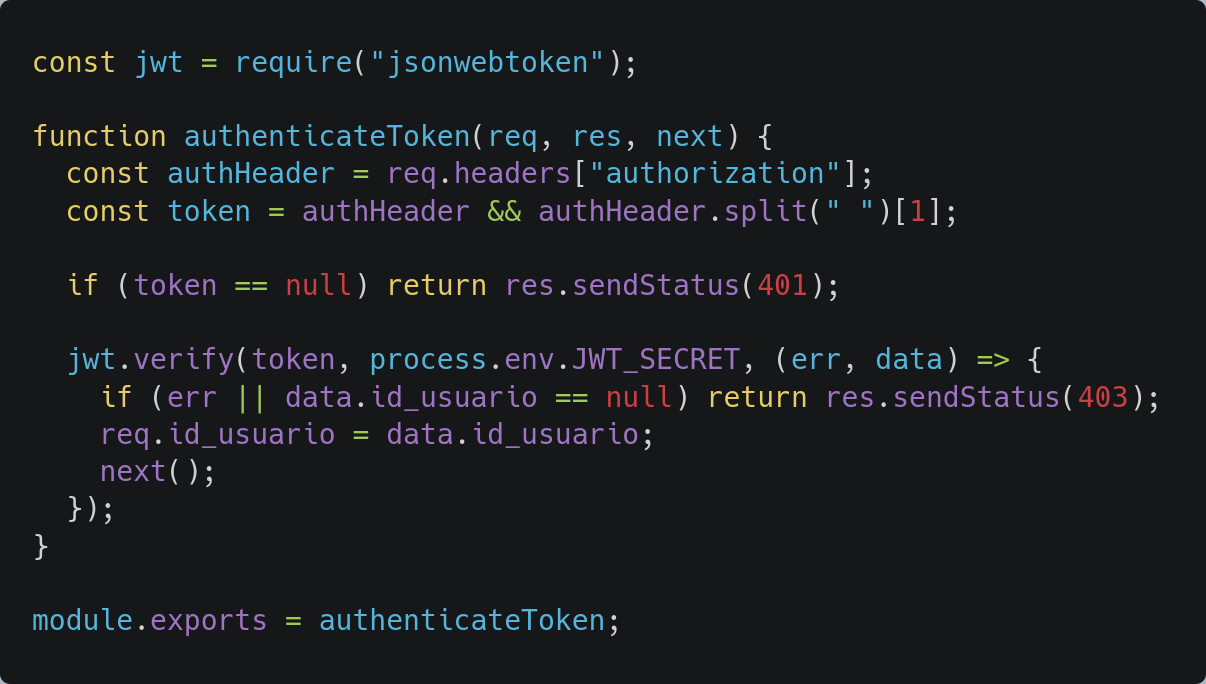
\includegraphics[width=0.8\textwidth]{./dados/figuras/authMiddleware}
	\fonte{Autor}
	\label{fig:auth}
\end{figure}
\pagebreak

O outro middleware criado tem como objetivo assegurar que um usuário possa consultar apenas as configurações pelas quais seja responsável. Isso é feito utilizando o identificador do usuário, presente no \textit{payload} do \textit{token} JWT, conforme a figura \ref{fig:configMiddleware}. Caso o usuário não tenha um vínculo com a configuração que está tentando acessar, a requisição é bloqueada.

\begin{figure}[!htb]
	\centering
	\caption{Middleware de validação da configuração}
	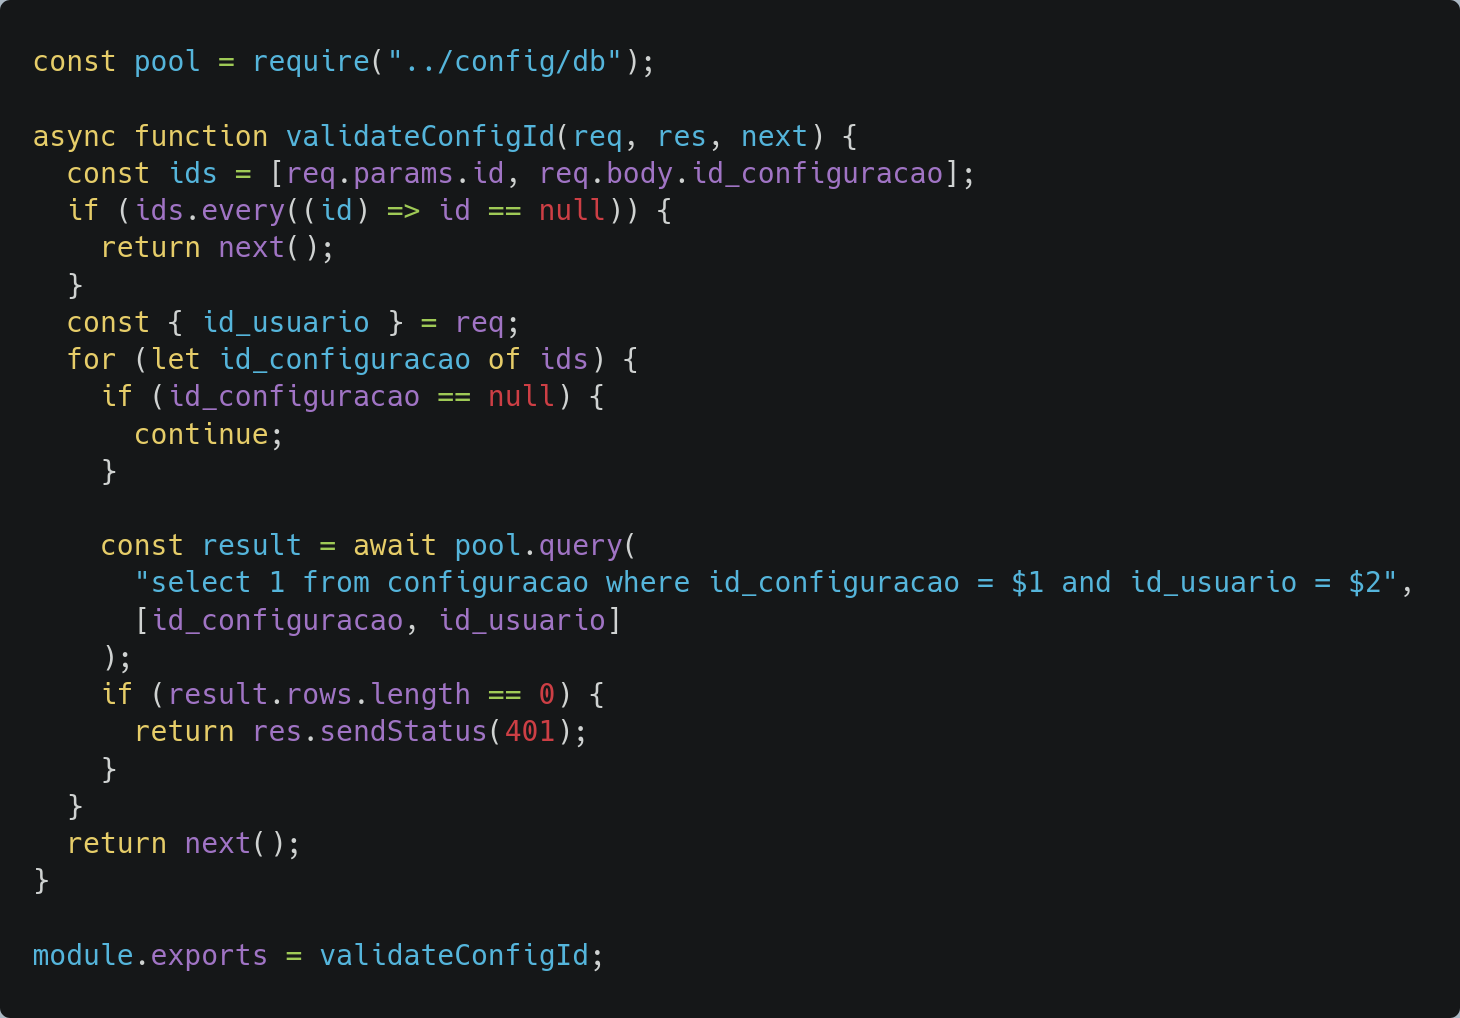
\includegraphics[width=0.8\textwidth]{./dados/figuras/configMiddleware}
	\fonte{Autor}
	\label{fig:configMiddleware}
\end{figure}
\pagebreak


